\section{Historical Costs, Stops, Control, and Target-Work Budgets}
\label{supp:history}
\subsection{Early four-system inventory and unchanged estimators}
\label{supp:historical_inventory}
The historical inventory uses MacBook Air M4/Metal (llama.cpp b10809), Core Ultra 9 275HX plus RTX 5070 Ti Laptop/CUDA (b10839), Core i5-13400 plus Arc B570/Vulkan0 (b10839), and Core Ultra X7 358H plus Arc B390/Vulkan0 with an OpenVINO draft. Qwen3-8B Q8\_0 is the target. Draft is Qwen3-0.6B Q8\_0 except the symmetric INT4 OpenVINO adapter. Hardware, OS, backend, placement and frontend vary jointly. The inventory is not a hardware-only comparison or a common energy/latency ranking.

Table~\ref{tab:historical_cost} reports the completed historical campaigns. M4's representative 24Q and separately preregistered HumanEval30 have opposite measured outcomes in distinct sessions. This does not identify a workload-only cause. Early MLX precision/correctness failures are separate from the final Q8\_0 Metal configuration. RTX historical CPU-to-GPU and same-GPU controls retain different integration costs. B570's formal failure triggers its stop; a later six-prompt serial text probe passes 18/18, whereas its full 30-prompt serial text comparison reaches only 60/90. Remote-interaction-contaminated diagnostic observations are excluded from the final cells. Legacy ``exact'' labels do not upgrade the text contract.

\begin{table*}[t]\centering\small
\caption{Historical latency outcomes under their original contracts. Intervals are descriptive and source-specific. Text agreement is not a direct-ID certificate.}
\label{tab:historical_cost}
\begin{tabularx}{\linewidth}{@{}Xrrl@{}}\toprule
Campaign & Speed & Interval & Agreement\\\midrule
M4 representative 24Q & 0.842 & [0.809,0.877] & 72/72 text\\
M4 HumanEval30 & 1.387 & [1.351,1.422] & 90/90 text\\
RTX CPU draft, HumanEval30 & 0.404 & [0.390,0.418] & 90/90 text\\
RTX same-GPU draft, HumanEval30 & 0.650 & [0.629,0.673] & 90/90 text\\
B570 serialized fallback & 0.3087 & [0.2927,0.3246] & 60/90 text\\
358H CPU stateful, HumanEval30 & 0.733915 & [0.692920,0.771090] & 90/90 IDs\\
358H NPU stateful, HumanEval30 & 0.351663 & [0.332595,0.368949] & 90/90 IDs\\\bottomrule
\end{tabularx}
\end{table*}

Historical M4 24Q takes a within-prompt GM of three paired ratios, then resamples prompts 10,000 times with Python Random seed 20260907 and sorted draw indices 249/9749. M4 HumanEval uses the same within-prompt aggregation but 100,000 draws, seed 20260910 and indices 2500/97499. Historical RTX uses 10,000 draws, seed 20260910, indices 249/9749. B570 fallback uses 10,000 draws, seed 20260910 and indices 250/9750 in archived insertion order. Sorting tasks changes its finite-seed endpoints and is not substituted. 358H uses prompt medians of three paired ratios, 10,000 draws, NumPy default\_rng seed 20260919 and .025/.975 quantiles. These policies are not replaced by late RTX's ratio-of-medians estimator.

\subsection{Target-forward proxies and energy boundaries}
\label{supp:historical_proxies_energy}
The historical target-only proxy is
\[
V_k^{\mathrm{micro}}(n,e)=T_{\mathrm{target\ forward}}(k,n,e)/T_{\mathrm{target\ decode}}(1,n).
\]
It omits drafting and can omit correction/bonus, state work and complete target-round bookkeeping. Table~\ref{tab:proxy_lookup} retains every context cell. Their ranges span contexts rather than uncertainty intervals. The historical RTX HumanEval/106 diagnostic repeats a same-position argmax change from 2790 to 2629 three times, with a separately instrumented same-commit margin moving from $+0.080948$ to $-0.126457$. It is shape-sensitive evidence in that configuration, not a unique kernel cause or a formal timing observation.

\begin{table}[ht]\centering\small
\caption{Frozen target-forward proxy lookup. These are neither complete target-round cost nor integrated speed. Historical text agreement applies only under each original comparator.}
\label{tab:proxy_lookup}
\begin{tabular}{@{}lrr@{}}\toprule
Path & Context & $V_2^{\mathrm{micro}}$\\\midrule
M4 Metal & 512 & 1.022182\\
M4 Metal & 2048 & 1.076126\\
M4 Metal & 8192 & 1.032264\\
RTX batched & 0 & 1.009030\\
RTX batched & 256 & 0.983148\\
RTX serialized & 0 & 2.430996\\
RTX serialized & 256 & 2.137011\\
B570 fast & 512 & 1.242576\\
B570 fast & 2048 & 1.637295\\
B570 serialized & 512 & 1.982668\\
B570 serialized & 2048 & 1.991707\\\bottomrule
\end{tabular}
\end{table}

M4 HumanEval energy measures the Silemetry CPU+GPU+ANE package aggregate, excluding separate DRAM. Fixed-$k=2$ package efficiency is $1.013\times$ with interval $[0.990,1.034]$, so improvement is not established. The registered secondary $p_{\min}=0.9$ condition has $1.041\times$ $[1.018,1.065]$, without replacing the primary or establishing material added speed. The corrected synthetic ceiling was registered but not executed; earlier synthetic diagnostics are not a substitute.

RTX board and CPU-package sensors are distinct domains, and follow-up process windows include loading; no formal serial HumanEval energy comparison is claimed. B570 fallback measures adapter-board efficiency $0.302\times$ $[0.285,0.320]$, without CPU package or wall power, and its output failure confines the result to diagnosis. 358H has no qualified end-to-end energy boundary. No late runtime repair energy, common system-energy ranking or concurrent-throughput result is inferred.

\subsection{Fresh direct-ID gates and independent latency arm}
\label{supp:historical_id_gates}
Fresh RTX direct-ID v2 has 270 executions on 30 HumanEval tasks, three conditions and three repeats. Batched $k=2$ reaches 75/90 (25/30 wholly equal prompts) and is blocked; serialized reaches 90/90 and qualifies. Mismatching first indices are /64:114, /106:65, /119:17, /128:41 and /129:21, stable across repeats. All conditions repeat stably. The initial v1 transport study retains 83 executions, 82 valid, and no qualification result: full-log UTF-8 decoding fails on a partial draft fragment after native exit zero. V2 changes observational byte transport and restarts the whole frozen schedule; it imports no v1 formal pairs. The final report stored at the repository's v1 path is a copy of the completed v2 report; it does not document v1 completion.

B570's separate fresh direct-ID campaign also completes 270 executions: fast reaches 60/90 (20/30 prompts), serialized 78/90 (26/30), and both are blocked. Historical fast 45/90 and serial 60/90 are unchanged text-path counts. An initial metadata decoding launch fails before inference with zero formal executions; authorized direct execution of the unchanged frozen runner produces the full campaign. No formal speed is inferred from operational elapsed fields. Neither new gate retroactively qualifies old timings.

The independent RTX matched-latency arm has 180 fresh timing observations and 90/90 fresh complete-ID agreements on 30 tasks. Serialized speed is $0.645816\times$, interval $[0.629802,0.659884]$, zero of 30 faster. Condition order uses seed 2026093001; the 10,000 prompt-bootstrap draws use seed 2026093002 and linear percentiles. Native QPC timing starts after synchronized target/draft prefill and covers per-request sampler/state work, drafting, verification, acceptance/correction/bonus, rollback, synchronization, logging/response and slot release. Load and teardown are excluded. Chrono shares the host oscillator; it is not an independent physical clock. The empty-hook probe bounds clock-call overhead, not all logging overhead. The fresh frontend is compiled with Clang 21.1.0 over retained CUDA libraries; OS build 26300 differs from the earlier direct-ID OS26200. These facts preclude synthetic pairing with prior qualification.

\subsection{V3 stop, V4 recovery, and protocol amendment}
\label{supp:v3_v4}
V3 plans 576 formal condition/repetition rows over 24 tasks. It delivers 126 valid prefix rows: 72 pre-live and 54 cost, with two failures and 448 unreached rows. Native HumanEval/59 emits 128 committed IDs ending at EOG and reports both limit and EOS. The frozen parser accepts only one marker and stops. Exit zero is not sufficient to make capture valid. A-live receives zero formal runs; complete formal accuracy, speed and interval are unavailable. Engineering qualification's 400 runs and parser-negative fixtures do not repair the missing formal endpoint branch. Old failures remain sealed.

V4 fixes that observational endpoint handling under a new freeze, accepting the ordered complete EOS-at-cap case while rejecting contradictory, reversed, duplicate or missing markers. Its 19-task panel initially comprises the remaining project-unused HumanEval inputs; subsequent reuse is exposed. It retains 228 pre-live predictor records and adds 57 native live and 171 fresh timing observations: 456 complete formal condition rows. Prediction closure is described in Section~\ref{supp:diagnosis}. The cost arm uses one timer executable and balanced order, each condition appearing in each order position 19 times. Batched qualification remains 51/57 and has no admissible speed/interval. Global serialization qualifies 57/57 but yields $0.677351\times$ $[0.661653,0.691812]$, zero of 19 faster. Median task absolute times are 1.607 s target and 2.332 s serial; their ratio is not the paired GM. The interval uses 10,000 paired-row draws, seed 2026100204 and linear quantiles.

The V4 numerical sources and assets remain frozen, but a fan-curve change triggers the original strict host-hash stop before live outcomes. Authorized continuation preserves the original \texttt{PROVENANCE\_INVALID} records, repeated predictor checks and the amendment. Fan/lighting differences become permitted; non-fan material settings remain strict. Predictor data are reused, not relabeled as a fresh untouched cohort. Fan controls stay fixed during the fresh timing arm, with snapshots retained, but can still affect latency. The campaign completed under the disclosed amendment; the original no-deviation host policy did not pass. Instrumented post-prefill-to-slot-release time is distinct from the later server generation field and cannot form a common optimization curve.

\subsection{RTX efficiency screening}
\label{supp:rtx_efficiency_pilot}
The early FA-on/UB512 four-probe pilot qualifies small-model $k=2$ and $k=4$, with request/generation speeds $1.277\times/1.324\times$ and $1.492\times/1.572\times$. Each FA/UB setting has its own ordinary reference; global UB changes several phases. Expansion to HumanEval/0--7 preserves every failure: final small-model $k=2$ qualifies 18/24, fragment drafting 21/24 and the mixed strategy 15/24. A mixed result producing 18 rather than the reference 87 IDs is invalid as a speed claim. $k=2$ repairs /5 but introduces /2; /6 remains divergent. The campaign has 300 formal requests and 48 excluded warmups. Synthetic favorable cases do not support the current headline.

\subsection{M4 formal control and oracle opportunity}
\label{supp:m4_control}
The M4 Guard measures cumulative charged generation time per committed ID, including seed/correction/bonus and excluding rejected proposals. It starts on Always speculation and can fall back permanently after a completed round, reconciling invalid target/draft suffixes first. Calibration freezes target cost per ID and selects \texttt{E8\_M000} from a nine-candidate grid with rounds $\{2,4,8\}$ and margins $\{0,0.05,0.10\}$. Exactness and calibration regret select the rule; ties use frozen overhead/exploration/margin/ID rules. Disjoint calibration, qualification and held-out task IDs prevent held-out retuning. Online decisions receive no future length, task family, request-specific target latency or oracle answer.

The registered post-prefill clock includes generation initialization, seed sampling, draft/target work, synchronization, reconciliation, control and transition. Load, sampler/speculator setup, initial prefill and the speculative begin hook precede it. This is not whole HTTP request latency. The formal campaign has 60 held-out tasks, 30 each HumanEval and Spec-Bench, three conditions and three repeats. Always and Guard each qualify 180/180 IDs. Table~\ref{tab:m4_strata} gives their original overall and family estimates.

% Generated by scripts/reconstruct.py from frozen exports.
\begin{table*}[t]\centering\small
\caption{M4 formal post-prefill baseline/candidate speeds from three-repeat condition medians. Family strata are descriptive.}\label{tab:m4_strata}
\begin{tabular}{@{}lrrr@{}}\toprule
Panel & Tasks & Target/Always & Target/Guard\\\midrule
Overall & 60 & 1.346894 & 1.311387\\
HumanEval & 30 & 1.570011 & 1.554690\\
Spec-Bench & 30 & 1.155485 & 1.106160\\
\bottomrule\end{tabular}

\end{table*}


The primary 10,000-draw bootstrap uses Python Random seed 20260924 in held-out order, with one continued stream for target/Guard, target/Always and Guard/oracle. The paired Guard/Always secondary replay starts a fresh stream of the same seed and uses linear percentiles; it gives latency $1.027076$ $[1.012956,1.043559]$, with Guard faster on 24 and Always on 36 tasks. It is post-study, not the original preregistered endpoint. A separate family-stratified sensitivity uses seed 2026100101, 10,000 draws and HumanEval-then-Spec-Bench order, giving $[1.0135,1.0423]$; it leaves the original intervals unchanged.

The per-task two-fixed-mode oracle improves the measured interval by factor $1.0006919671$ relative to Always. The implied latency reduction is $1-1/1.0006919671=0.0006914886$, approximately 0.069149\%. Only Spec-Bench/559 and /95 favor target-only: target times are 11.9085 and 10.9203 s; Always/target latencies 1.0270 and 1.0150; Guard/target 1.0215 and 1.0029. This finite hindsight opportunity is not a bound on all intra-request policies.

A loop-variable shadowing defect records a build-manifest digest in the intended calibration-freeze field. Recovery verifies the actual freeze, source/model/calibration/policy hashes and formal-start links, retaining error markers and the original pipeline \texttt{STOPPED} metadata. It does not retune the policy or mutate measurements. Recorded Git order is not a trusted external timestamp. The resolved metadata defect does not change the formal experiment's completion status.

\subsection{358H state interface, threshold gate, and conditional budgets}
\label{supp:358h_budgets}
The 358H stateful runner is complete; the preceding preflight scaffold was empty and blocked. It keeps the target's low-level context between rounds and charges validation, rejected-suffix rollback, correction/bonus and synchronization within complete target work. Every OpenVINO proposal call receives the full committed prefix. The synchronous region combines replay/reconstruction and proposal, with no separate measurements of those terms.

A prior proxy threshold study passes 18 direct-ID sanity pairs and admits borderline context points, using a favorable zero residual $T_x$, fixed progress assumptions and seed 20260919, 10,000 empirical draws. It predicts eligibility, not achieved integrated speed. CPU central/optimistic speeds at contexts512/2048/8192 are 0.903680/1.355520, 0.884843/1.327264 and 0.755946/1.133919. NPU values are 0.905553/1.358329, 0.903804/1.355706 and 0.839618/1.259427. The subsequent actual stateful CPU/NPU speeds in Table~\ref{tab:historical_cost} are lower and qualified, with zero of 30 prompts faster on either path.

Table~\ref{tab:358h_accounting} retains measured progress, components and distinct ceiling estimators. Both paths commit 11,520 IDs, over 4,677 CPU and 4,686 NPU rounds. Arithmetic-total accounting gives normalized $(D,R,X)=(0.4304,2.9767,0.00124)$ CPU and $(4.1251,2.9435,0.00130)$ NPU. These values reproduce total-time ratios, not prompt GMs. Target-only ceilings assume unchanged baseline, target work and progress with all other nonnegative cost removed.

Let $B_{ij}$ be matched target-only time and $T_{ij}$ measured complete target work for prompt $i$ and repetition $j$. If optimized speculative time retains this target work and only reduces the other nonnegative costs, its speed $S'_{ij}$ is at most $B_{ij}/T_{ij}$. Monotonicity of the median and geometric mean then gives the bound under the original prompt estimator:
\begin{equation}
\operatorname{GM}_{i}\operatorname{median}_{j} S'_{ij}
\leq \operatorname{GM}_{i}\operatorname{median}_{j}(B_{ij}/T_{ij}).
\label{eq:floor}
\end{equation}
For a uniform fractional reduction $\delta$ in target work, the corresponding zero-other-work ceiling increases by $1/(1-\delta)$. If its original value is $F<1$, parity therefore requires $\delta\geq 1-F$. Table~\ref{tab:358h_accounting} reports this necessary budget separately for the prompt and pooled-total estimators. It assumes fixed baseline and committed progress; changing either requires fresh qualification and measurement.

% REVISION_ADDITION_BEGIN: 358H conditional budget visual explanation
Figure~\ref{fig:358h_budget} places the measured prompt-estimator speeds beside their conditional ceilings and the necessary target-work cuts. The pooled-total estimator remains separate in Table~\ref{tab:358h_accounting}.

\begin{figure*}[t]
\centering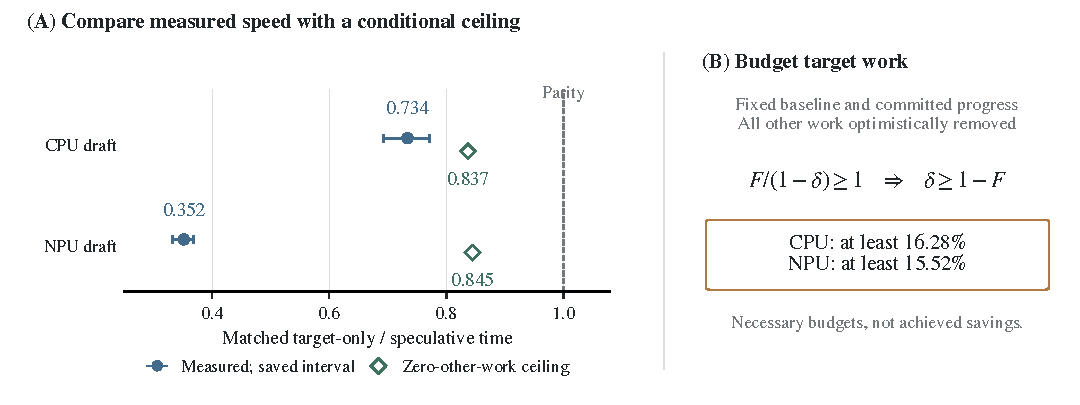
\includegraphics[width=\linewidth]{figures/figure_S2_358h_budget.pdf}
\caption{358H measured speed and a conditional optimization budget. (A) Filled circles and bars show the saved speed estimates and descriptive prompt-bootstrap intervals; open diamonds show arithmetic ceilings if all other nonnegative work were removed while baseline, target work and committed progress stayed fixed. All points use the original geometric mean of 30 prompt medians of three paired ratios. Ceiling markers have no confidence intervals. (B) Reaching parity in that optimistic case requires a uniform target-work cut of at least $1-F$, where $F$ is the original ceiling. These are necessary budgets, not achieved savings or an impossibility claim about NPUs. The 180-row original-host ceiling audit remains inherited.}
\label{fig:358h_budget}
\end{figure*}
% REVISION_ADDITION_END

\begin{table*}[t]\centering\small
\caption{358H measured accounting and conditional zero-other-work ceilings. Percentages describe the saved synchronous regions; prompt and pooled estimators remain distinct.}
\label{tab:358h_accounting}
\begin{tabular}{@{}lrr@{}}\toprule
Quantity & CPU draft & NPU draft\\\midrule
Committed IDs per round & 2.463117 & 2.458387\\
Replay plus proposal share (\%) & 12.6273 & 58.3474\\
Complete target-work share (\%) & 87.3365 & 41.6342\\
Residual share (\%) & 0.0363 & 0.0184\\
Actual pooled-total speed & 0.7227 & 0.3477\\
Pooled-total ceiling & 0.8274529834 & 0.8351858524\\
Prompt-estimator ceiling & 0.8372192092 & 0.8448401086\\
Necessary uniform target cut, prompt (\%) & 16.278079 & 15.515989\\
Necessary uniform target cut, pooled (\%) & 17.254702 & 16.481415\\\bottomrule
\end{tabular}
\end{table*}

No prompt-median ceiling reaches parity; maximum prompt ceilings are 0.9736196764 CPU and 0.9999089575 NPU. One NPU repetition has $B/T=1.000163695$, so not every individual run-level ceiling is below one. The budgets are necessary arithmetic reductions under fixed progress, not achieved optimizations or proof against NPUs. A persistent-state/wider-target candidate stops at qualification: CPU restore/reconcile correctness is unavailable under the tested representation, and the frozen dynamic-shape NPU IR lacks the required state-capable path. Same-prefix target-only and proposal-replay diagnostics identify greedy divergence but not a unique rollback bug. No formal runtime performance or energy result exists for that failed candidate; the completed earlier Phase-3 costs remain valid under their own contract.

